\documentclass[../m180main.tex]{subfiles}
\graphicspath{{\subfix{../figures/}}}

\begin{document}

\chapter{The Advection Equation}
\section{Derivation: Traffic Flow}
Consider a one-dimensional freeway with no entrances or exits, and let $\rho(x,t)$ denote the mass density of cars at a given position and time.
We'll build a model that describes the evolution of $\rho$ on a stretch of freeway with endpoints $x=a$ and $x=b$.
First note that the total mass $M(t)$ of cars on this stretch and its derivative are given by
\[ M(t) = \int_{a}^{b} \rho(x,t) \,dx, \qquad \frac{dM}{dt} = \int_{a}^{b} \frac{\pa \rho}{\pa t} \,dx, \]
where by a theorem of Leibniz the time derivative can be brought inside of the integral when $\rho$ and $\rho_t$ are both continuous.
Now, we can get another independent expression for $dM / dt$ by looking at the boundaries of our stretch of freeway---define $q(x,t)$ to be the rightward mass flux through a given point, so
\[ \frac{dM}{dt} = q(a,t) - q(b,t) = - \int_{a}^{b} \frac{\pa q}{\pa x} \,dx. \]
By equating our two expressions we get the equation
\[ \int_{a}^{b} \left[ \frac{\pa \rho}{\pa t} + \frac{\pa q}{\pa x} \right] dx = 0; \]
since this works for arbitrary $a,b$, the integrand must be zero and
\[ \rho_t + q_x = 0. \]
This is what we call the transport equation (or conservation law) for our setup.
It does a great job at conveying what's physically happening on the freeway at each point in space and time, but it's an equation in two potentially unrelated functions $\rho$ and $q$.
This isn't super conducive to an analytic solution.

\section{The Method of Characteristics}
Conveniently, we're often able to write the flux $q$ in terms of the density $\rho$.
For example, if the cars are traveling at a constant speed $c$ we have $q(x,t) = c \,\rho(x,t)$ and
\[ \rho_t + c \,\rho_x = 0. \]
This is called the advection (or convection) equation, and it's an important one.
But we'll focus our attention on the more general case in which $c$ may be a function of position and time---in particular, we will solve
\[ u_t + c(x,t) \,u_x = 0, \qquad u(x,0) = f(x) \]
for $-\infty < x < \infty$ and $t > 0$, where we've tacked on an initial condition for completion's sake.
We'll approach the problem using the method of characteristics.

The idea here is to find curves, called characteristics, on which the above PDE reduces to an ODE.
Specifically, we seek characteristics $x = x(t)$ on which $u(x(t), t)$ is constant in $t$.
We will exploit the fact that, under this condition,
\[ 0 = \frac{du}{dt} = \frac{\pa u}{\pa t} + \frac{\pa u}{\pa x} \frac{dx}{dt} = u_t + \frac{dx}{dt} u_x. \]
Comparing this with the PDE we started with reveals that $dx / dt = c(x,t)$, the solutions of which are the $x(t)$ we desire.
It turns out that substituting $\xi = x(0)$ and $\tau = t$ into our PDE reduces it to an ODE; solving it and undoing the substitution gives us the $u(x,t)$ we desired.
This is best illustrated via an example.

\begin{example}[Characteristics on an inhomogeneous PDE]
    Consider the PDE
    \[ u_t + c \,u_x = -u, \qquad u(x,0) = f(x) \]
    on $-\infty < x < \infty$ and $t > 0$.
    Despite this being an inhomogeneous equation, we can still solve it using characteristics!
    Using the chain rule to match the left-hand side of the PDE reveals that $dx / dt = c$, meaning our characteristics are
    \[ x(t) = ct + \xi \]
    for constant $\xi$.
    We'll substitute $\xi = x - ct$, $\tau = t$, and $U(\xi, \tau) = u(x,t)$; the relevant derivatives are
    \begin{align*}
        \frac{\pa u}{\pa x} &= \frac{\pa U}{\pa \xi} \frac{\pa \xi}{\pa x} + \frac{\pa U}{\pa \tau} \frac{\pa \tau}{\pa x} & \frac{\pa u}{\pa t} &= \frac{\pa U}{\pa \xi} \frac{\pa \xi}{\pa t} + \frac{\pa U}{\pa \tau} \frac{\pa \tau}{\pa t} \\
        &= \frac{\pa U}{\pa \xi}, & &= -c \frac{\pa U}{\pa \xi} + \frac{\pa U}{\pa \tau}.
    \end{align*}
    Substituting these into our PDE gives
    \[ \frac{\pa U}{\pa \tau} = -U, \]
    and we conclude that $U(\xi, \tau) = A(\xi) \,e^{-\tau}$ for some function $A$.
    After the substitution is undone we're left with $u(x,t) = A(x - ct) \,e^{-t}$, and applying the initial condition gives
    \[ u(x,t) = f(x - ct) \,e^{-t}. \]
\end{example}

Note that, despite our method for solving inhomogeneous PDEs being very similar to the one we have for homogeneous ones, in general there's a pretty big difference between the two.
Namely, the solutions to a homogeneous PDE comprise an infinite-dimensional vector space (so any linear combination of solutions is itself a solution) while those to an inhomogeneous PDE do not.

There's a couple of ways we might visualize the behavior of the solutions we get to a PDE of this form.
We could plot the characteristics in the $x$-$t$ plane for several different choices of $\xi$, or we could plot several different ``snapshots'' of our solution curve in the $x$-$u$ plane.
Both of these are simple in principle, but can be quite complicated to pull off for nonlinear PDEs.
More on that soon.

\section{Characteristics and Nonlinear PDEs}
Going back to our traffic model, it would make the most sense if speed depended on density.
In this case the flux looks like $q(\rho) = c(\rho) \rho$, and from the transport equation we get
\[ \rho_t + [c(\rho) \rho]_x = 0. \]
For our purposes, we'll say an individual car travels with phase velocity $c(\rho) = c_\star (1 - \rho / \rho_\star)$.
Substituting into the above equation gives
\[ \rho_t + c_\star \left( 1 - \frac{2\rho}{\rho_\star} \right) \rho_x = 0. \]
The coefficient on the $\rho_x$ is called the group velocity.
We might interpret it as the speed at which the cars, as a whole, tend to move through space.

We'll take $x \in \R$, $t > 0$, and $\rho(x,0) = f(x)$.
Applying the method of characteristics gives the ODE
\[ \frac{dx}{dt} = c_\star \left( 1 - \frac{2\rho}{\rho_\star} \right); \]
we'll call the right-hand side $v(\rho)$.
Solving gives the characteristics $x(t) = v(\rho) \,t + \xi$.
Substituting, solving, and un-substituting would give the solutions
\[ \rho(x,t) = f \big( x - v(\rho) \,t \big). \]
This would be great if it weren't for one glaring problem: $\rho$ is now given in terms of $\rho$.
To see how we might deal with this, let's look at a very simple initial condition,
\[ \rho(x,0) = \begin{cases} \rho_\star & x < 0, \\ 0 & x > 0. \end{cases} \]
The characteristics rooted at $x \neq 0$ are sketched below, on the left.
This clarifies that $\rho(x,t) = \rho_\star$ for $x < -c_\star t$ and $\rho(x,t) = 0$ for $x > c_\star t$, but we don't yet have any information about what happens in between.

\begin{center}
    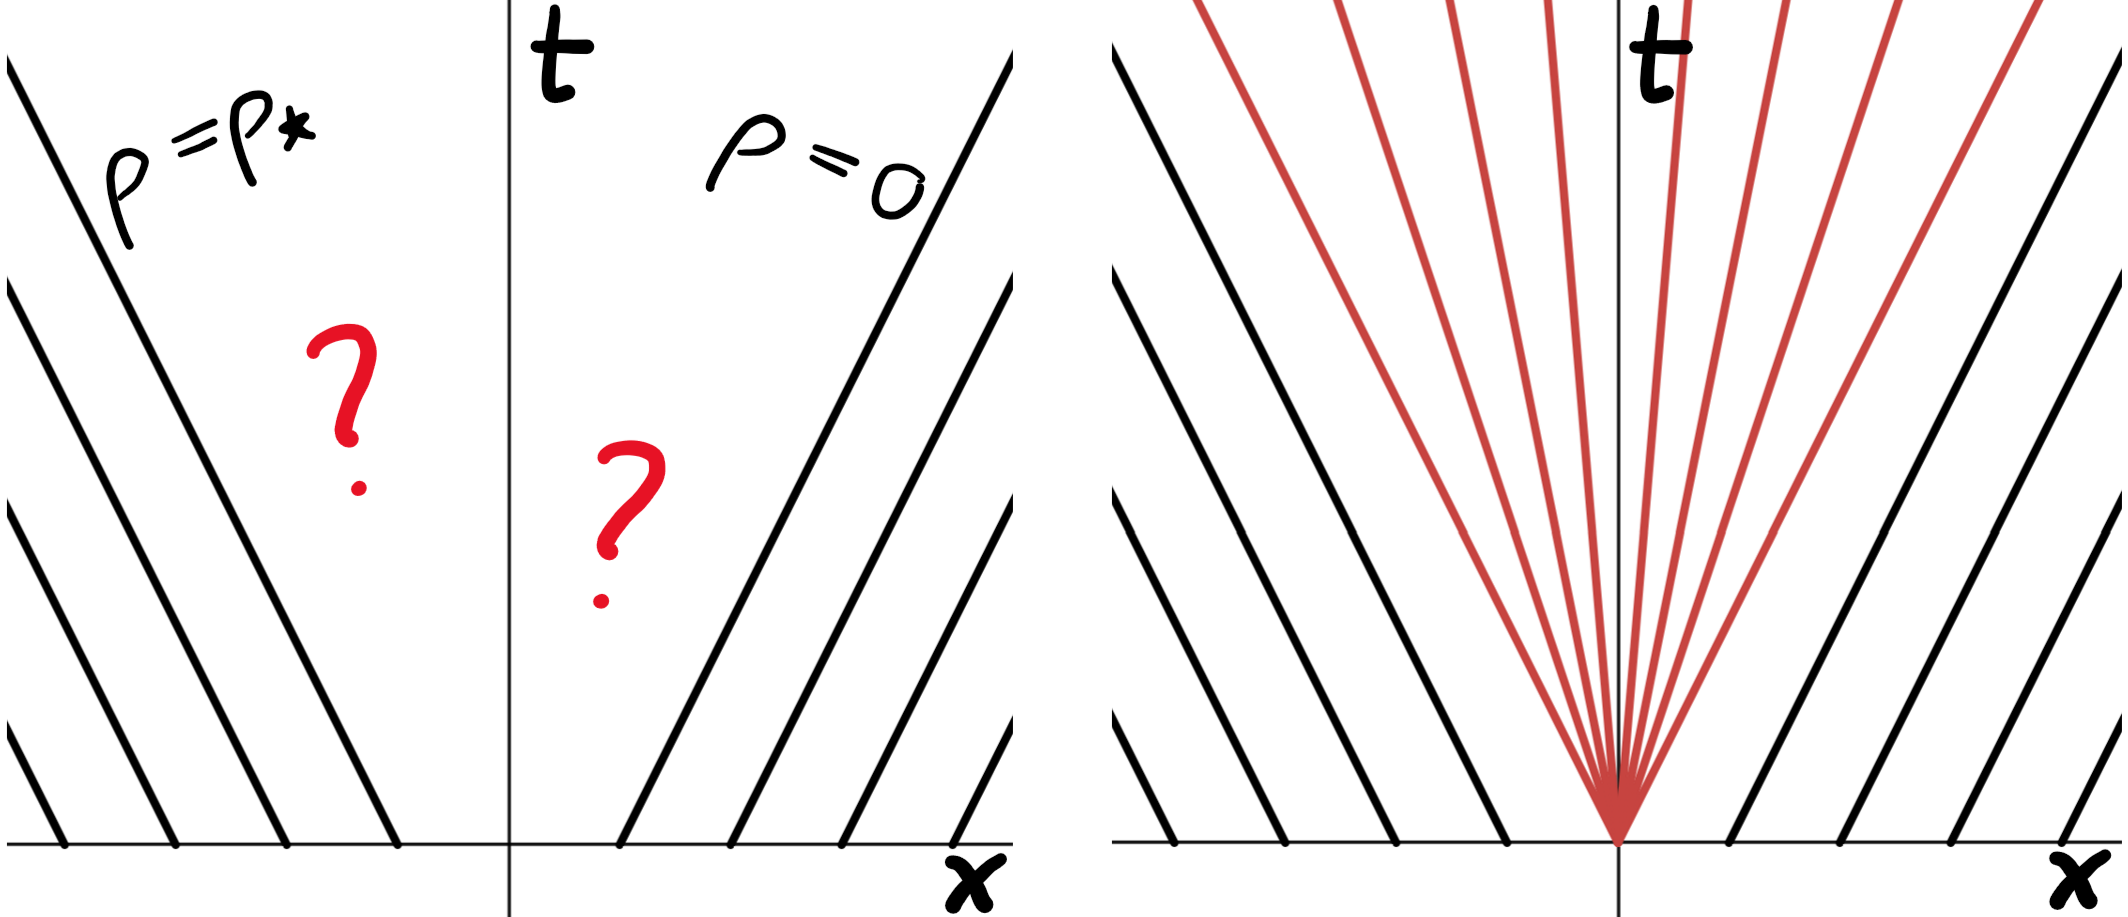
\includegraphics[width=0.85\textwidth]{rarefaction.png}
\end{center}

To resolve this we might imagine that our initial condition is actually smooth, our two pieces connected by a very thin logistic curve.
In this region $\rho$ varies from $\rho_\star$ to $0$, and the slopes of our characteristics 
\[ x(t) = c_\star \left( 1 - \frac{2\rho}{\rho_\star} \right) \]
vary from $-c_\star$ to $c_\star$.
These new characteristics are plotted above in red.
Solving for $\rho$ gives the solution to the PDE in the in-between region.

% To learn how to do this on inhomogeneous PDEs, go to grad school.

\section{Finite Difference Methods}
Now we'll look a little bit at numerical methods, in particular finite difference methods.
Our goal is to sketch a program to simulate solutions to the advection equation
\[ u_t + c u_x = 0, \qquad u(x,0) = f(x) \]
for $x \in (0, L)$ and $t \in (0, T)$.
Our domain will be split into chunks using fixed step sizes $\Delta x$ and $\Delta t$.
In this way, a position in space and time can be specified by two integer coordinates $j,n$---we'll use the notation
\[ u_j^n = u(j \Delta x, \, n \Delta t). \]
We'll often pack all of the position data for a given time into a vector $\mbf{u}^n$.
This will become useful to us very soon!
But for now we need to determine how we should approximate derivatives in this discretized space.
We have a few options for finite difference methods.
\begin{itemize}
    \item Forward difference.
    We start at $\mbf{u}^n$ and jump ahead to $\mbf{u}^{n+1}$.
    Here,
    \[ \frac{\pa u}{\pa t} \approx \frac{u_j^{n+1} - u_j^n}{\Delta t}. \]

    \item Backward difference.
    We start at $\mbf{u}^n$ and jump backward to $\mbf{u}^{n-1}$.
    \[ \frac{\pa u}{\pa t} \approx \frac{u_j^n - u_j^{n-1}}{\Delta t}. \]

    \item Centered difference.
    We jump between $\mbf{u}^{n-1}$ and $\mbf{u}^{n+1}$.
    \[ \frac{\pa u}{\pa t} \approx \frac{u_j^{n+1} - u_j^{n-1}}{2\Delta t}. \]
\end{itemize}
If we work with forward differences in both space and time then the advection equation becomes
\[ \frac{u_j^{n+1} - u_j^n}{\Delta t} + c \, \frac{u_{j+1}^n - u_j^n}{\Delta x} = 0 \]
with initial conditions $u_0^0, \ldots, u_k^0$.
Solving for $u_j^{n+1}$:
\[ u_j^{n+1} = u_j^n - \frac{c \,\Delta t}{\Delta x} \left( u_{j+1}^n - u_j^n \right). \]
The vector equation
\begin{align*}
    \mbf{u}^{n+1} &= \mbf{u}^n - c \frac{\Delta t}{\Delta x} A \mbf{u}^n \\
    &= \left( I - \frac{c \Delta t}{\Delta x} A \right) \mbf{u}^n
\end{align*}
describes this for all valid $j$, where
\[ A = \begin{bmatrix} -1 & 1 & 0 & \cdots & 1 \\ 0 & -1 & 1 & \cdots & 0 \\ 0 & 0 & -1 & \cdots & \vdots \\ \vdots & \vdots & \vdots & & \vdots \\ 0 & 0 & 0 & \cdots & 1 \\ 0 & 0 & 0 & \cdots & -1 \end{bmatrix}. \]
Note that the $1$ in the top-right corner encodes a periodic boundary condition $u(0,t) = u(L,t)$.
Now, $A$ has the sole eigenvalue $\lambda = -1$, meaning those of $I - \frac{c \Delta t}{\Delta x}$ are $\lambda = 1 + \frac{c \Delta t}{\Delta x}$.
Our solution is stable if $|\lambda| \leq 1$, so in our case the criterion is
\[ -2 \Delta x < c \Delta t < 0. \]
Since $\Delta x$ and $\Delta t$ are both positive, this method is never stable.
Other combinations may work, though!

\end{document}